% ============================================================================
%  MASTER RESULTS: Neural Network Track Extrapolation (V1–V4)
%  Author: G. Scriven (LHCb, Nikhef)
%  Date:   February 2026
% ============================================================================
\documentclass[11pt,a4paper]{article}

% ---- packages --------------------------------------------------------------
\usepackage[utf8]{inputenc}
\usepackage[T1]{fontenc}
\usepackage{lmodern}
\usepackage[margin=2.4cm]{geometry}
\usepackage{amsmath,amssymb,bm}
\usepackage{graphicx}
\usepackage{tikz}
\usetikzlibrary{positioning, arrows.meta, calc, decorations.pathreplacing, fit, shapes.geometric}
\usepackage{booktabs}
%\usepackage{multirow}  % not installed
\usepackage{xcolor}
\usepackage{hyperref}
\usepackage{caption}
\usepackage{subcaption}
\usepackage{float}
\usepackage{enumitem}
\usepackage{fancyhdr}
% siunitx not available; define lightweight replacements
\newcommand{\SI}[2]{#1\,\text{#2}}
\newcommand{\si}[1]{\text{#1}}
\newcommand{\num}[1]{#1}

% ---- colours ---------------------------------------------------------------
\definecolor{mlpblue}{HTML}{1F77B4}
\definecolor{pinngreen}{HTML}{2CA02C}
\definecolor{rkpinnorange}{HTML}{FF7F0E}
\definecolor{rk4red}{HTML}{D62728}
\definecolor{lightgray}{HTML}{F0F0F0}
\definecolor{darkgray}{HTML}{404040}

% ---- hyperref setup --------------------------------------------------------
\hypersetup{
  colorlinks=true,
  linkcolor=mlpblue,
  citecolor=pinngreen,
  urlcolor=rkpinnorange,
}

% ---- headers ---------------------------------------------------------------
\pagestyle{fancy}
\fancyhf{}
\fancyhead[L]{\small Neural Network Track Extrapolation}
\fancyhead[R]{\small V1--V4 Master Results}
\fancyfoot[C]{\thepage}

% ---- custom commands -------------------------------------------------------
\newcommand{\zfrac}{\zeta}
\newcommand{\dz}{\Delta z}
\newcommand{\qop}{q/p}
\newcommand{\vstate}{\mathbf{s}}
\newcommand{\vc}{\mathbf{c}}
\newcommand{\vB}{\vec{B}}
\newcommand{\IC}{\mathrm{IC}}
\newcommand{\tx}{t_x}
\newcommand{\ty}{t_y}
\DeclareMathOperator{\SiLU}{SiLU}

% ============================================================================
\begin{document}

% ---- title -----------------------------------------------------------------
\begin{center}
  {\LARGE\bfseries Neural Network Track Extrapolation\\[4pt]
   Master Results: V1\,--\,V4}\\[12pt]
  {\large G.~Scriven}\\[4pt]
  {\normalsize LHCb, Nikhef}\\[4pt]
  {\normalsize February 2026}
\end{center}
\vspace{6pt}
\hrule
\vspace{12pt}

\begin{abstract}
This document aggregates all mathematics, architecture details, results and
figures from four iterative versions of neural-network-based track
extrapolators developed for the LHCb experiment.  Three model families are
studied---plain multi-layer perceptrons (MLPs), physics-informed neural
networks (PINNs) with a residual formulation, and Runge-Kutta-structured
PINNs (RK-PINNs) with collocation losses.  The document provides a
self-contained treatment of the underlying physics, the residual output
theory that guarantees initial conditions, and the collocation training
strategy for the RK-PINN, together with complete numerical results across
all versions.
\end{abstract}

\tableofcontents
\newpage

% ============================================================================
\section{Introduction}\label{sec:intro}
% ============================================================================

A charged particle travelling through the LHCb dipole magnet follows a
curved path governed by the Lorentz force.  The standard method for
predicting where the particle ends up is fourth-order Runge-Kutta (RK4)
numerical integration, which requires many evaluation steps and magnetic
field lookups.

This project replaces RK4 with a \emph{neural network} that learns the same
input--output mapping in a single forward pass.

\paragraph{Input (6 numbers).}
\begin{equation}\label{eq:input}
  \mathbf{x}_{\mathrm{in}} = \bigl(\, x_0,\; y_0,\; \tx{}_0,\; \ty{}_0,\;
  \qop,\; \dz \,\bigr)
\end{equation}
where $(x_0,y_0)$ is the starting position in millimetres, $(\tx{}_0,\ty{}_0)$
are the track slopes $dx/dz$ and $dy/dz$, $\qop$ is charge divided by
momentum (\si{\per\mega\electronvolt}), and $\dz$ is the propagation distance
along $z$ (mm).

\paragraph{Output (4 numbers).}
\begin{equation}\label{eq:output}
  \mathbf{x}_{\mathrm{out}} = \bigl(\, x,\; y,\; \tx,\; \ty \,\bigr)
  \quad\text{at}\quad z = z_0 + \dz
\end{equation}

% ============================================================================
\section{The Physics}\label{sec:physics}
% ============================================================================

% ---------- Lorentz force ---------------------------------------------------
\subsection{Lorentz Force in the LHCb Parameterisation}

A charged particle in a magnetic field $\vB(x,y,z)$ obeys an ordinary
differential equation in $z$:
\begin{equation}\label{eq:lorentz}
  \frac{d}{dz}
  \begin{pmatrix} x \\ y \\ \tx \\ \ty \end{pmatrix}
  =
  \begin{pmatrix}
    \tx \\[4pt]
    \ty \\[4pt]
    \kappa\,\sqrt{1+\tx^2+\ty^2}\;\bigl[\tx\ty B_x
      - (1+\tx^2)\,B_y + \ty B_z\bigr] \\[4pt]
    \kappa\,\sqrt{1+\tx^2+\ty^2}\;\bigl[(1+\ty^2)\,B_x
      - \tx\ty B_y - \tx B_z\bigr]
  \end{pmatrix}
\end{equation}
with
\begin{equation}\label{eq:kappa}
  \kappa = \frac{q}{p}\,c_{\mathrm{light}}
  = \frac{q}{p}\times 2.998\times10^{-4}
  \;\si{\milli\metre\per(\mega\electronvolt\,\tesla)}
\end{equation}

The key features of this system:
\begin{itemize}[nosep]
  \item Positions ($x,y$) evolve linearly in $z$ through the slope terms.
  \item Slopes ($\tx,\ty$) change due to the magnetic field---this is the
        bending.
  \item The coupling constant $\kappa\propto q/p$ means low-momentum
        particles bend more.
\end{itemize}

% ---------- Dipole field ---------------------------------------------------
\subsection{The LHCb Dipole Field}

The vertical field component $B_y$ is \emph{not} uniform---it varies by a
factor of ${\sim}3$ across the magnet:

\begin{table}[H]
\centering
\caption{Approximate $B_y$ along the beam axis.}
\label{tab:field}
\begin{tabular}{@{} r r c @{}}
\toprule
$z$ (mm) & $B_y$ (T) & Relative curvature \\
\midrule
0    & 1.10 & $1.65\times$ \\
2000 & 0.95 & $1.43\times$ \\
4000 & 0.70 & $1.05\times$ \\
6000 & 0.50 & $0.75\times$ \\
8000 & 0.40 & $0.60\times$ \\
\bottomrule
\end{tabular}
\end{table}

This spatial variation is the single most important factor in the design of
neural-network extrapolators: any model that cannot represent position-dependent
curvature will inevitably fail.

% ---------- Taylor expansion -----------------------------------------------
\subsection{Taylor Expansion of a Trajectory}\label{sec:taylor}

Expanding the position to second order:
\begin{equation}\label{eq:taylor}
  x(z) = x_0 + \tx{}_0\,\dz
       + \frac{1}{2}\left.\frac{d^2 x}{dz^2}\right|_{z_0}\!\!(\dz)^2
       + \mathcal{O}(\dz^3)
\end{equation}
\begin{itemize}[nosep]
  \item \textbf{Linear term} ($\tx\!\cdot\!\dz$): straight-line
        extrapolation.
  \item \textbf{Quadratic term} (${\propto}\,\kappa\,B_y$): magnetic
        bending.
  \item \textbf{Higher-order terms}: field variation along the path.
\end{itemize}

A model whose output is linear in the propagation fraction $\zfrac$ captures
only the first term.  The quadratic bending---which can amount to hundreds
of millimetres for a \SI{20}{GeV} track over \SI{8}{\metre}---is missed
entirely.

% ============================================================================
\section{Model Architectures}\label{sec:arch}
% ============================================================================

Three families of neural network were studied.  This section describes each
architecture and its mathematical formulation.

% ---------- MLP  -----------------------------------------------------------
\subsection{MLP (Multi-Layer Perceptron)}\label{sec:mlp}

A plain feedforward network with no physics constraints:

\begin{equation}\label{eq:mlp}
  \hat{\mathbf{y}} = W_{N+1}\,\sigma\!\bigl(
    W_N\,\sigma\!\bigl(\cdots\sigma(W_1\,\mathbf{x}_{\mathrm{in}} + b_1)
    \cdots\bigr) + b_N\bigr) + b_{N+1}
\end{equation}
where $\sigma$ is the SiLU activation $\sigma(x)=x/(1+e^{-x})$.

\begin{figure}[H]
\centering
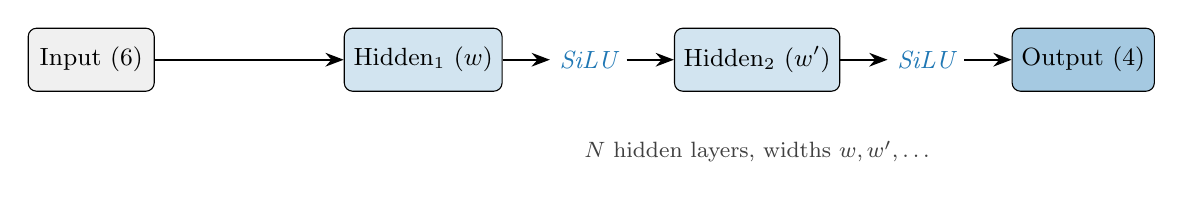
\begin{tikzpicture}[
  node distance=1.2cm and 2.4cm,
  layer/.style={draw, rounded corners=3pt, minimum width=1.6cm,
                minimum height=0.8cm, font=\small},
  arrow/.style={-Stealth, thick},
]
  % Input
  \node[layer, fill=lightgray] (in) {Input (6)};
  % Hidden 1
  \node[layer, fill=mlpblue!20, right=of in] (h1) {Hidden$_1$ ($w$)};
  % Activation
  \node[right=0.6cm of h1, font=\small\itshape, text=mlpblue] (a1) {SiLU};
  % Hidden 2
  \node[layer, fill=mlpblue!20, right=0.6cm of a1] (h2) {Hidden$_2$ ($w'$)};
  % Activation 2
  \node[right=0.6cm of h2, font=\small\itshape, text=mlpblue] (a2) {SiLU};
  % Output
  \node[layer, fill=mlpblue!40, right=0.6cm of a2] (out) {Output (4)};
  % Arrows
  \draw[arrow] (in) -- (h1);
  \draw[arrow] (h1) -- (a1);
  \draw[arrow] (a1) -- (h2);
  \draw[arrow] (h2) -- (a2);
  \draw[arrow] (a2) -- (out);
  % Label
  \node[below=0.5cm of h2, font=\footnotesize, text=darkgray]
    {$N$ hidden layers, widths $w, w', \ldots$};
\end{tikzpicture}
\caption{MLP architecture.  Input is the full 6-dimensional state
  including $\dz$; output is the 4-dimensional final state.}
\label{fig:mlp_arch}
\end{figure}

\paragraph{Loss function.}
Pure mean-squared error between predicted and true final states:
\begin{equation}\label{eq:mlp_loss}
  \mathcal{L}_{\mathrm{MLP}} =
  \frac{1}{B}\sum_{i=1}^{B}\bigl\|\hat{\mathbf{y}}_i - \mathbf{y}_i\bigr\|^2
\end{equation}

% ---------- PINN  ----------------------------------------------------------
\subsection{PINN (Physics-Informed Neural Network)}\label{sec:pinn}

\subsubsection{The Residual Formulation}\label{sec:residual}

The central idea of the PINN is to \emph{guarantee} the initial condition
by construction.  Define the fractional propagation coordinate:
\begin{equation}\label{eq:zfrac}
  \zfrac = \frac{z - z_0}{\dz} \in [0,\,1]
\end{equation}

The PINN output is then:
\begin{equation}\label{eq:pinn_residual}
  \boxed{\;
    \vstate(\zfrac) = \vstate_0 + \zfrac \cdot
    \underbrace{\mathcal{N}_\theta\!\bigl(x_0, y_0, \tx{}_0, \ty{}_0,
    \qop\bigr)}_{\text{correction vector }\vc}
  \;}
\end{equation}

where $\vstate_0 = (x_0, y_0, \tx{}_0, \ty{}_0)$ is the initial state (the
``IC''), $\mathcal{N}_\theta$ is a neural network with parameters $\theta$,
and $\vc$ is a single correction vector that does \emph{not} depend on $\zfrac$.

\begin{figure}[H]
\centering
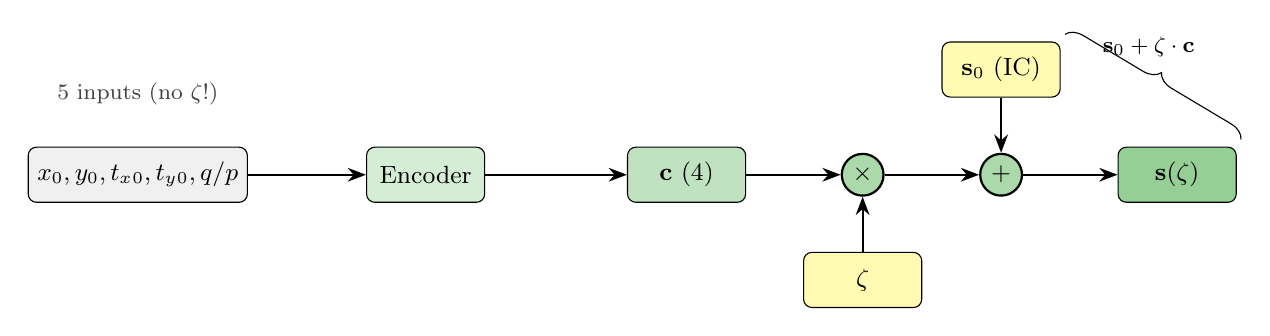
\begin{tikzpicture}[
  node distance=0.9cm and 1.8cm,
  layer/.style={draw, rounded corners=3pt, minimum width=1.5cm,
                minimum height=0.7cm, font=\small},
  op/.style={draw, circle, inner sep=2pt, font=\small, thick},
  arrow/.style={-Stealth, thick},
  darrow/.style={-Stealth, thick, dashed},
]
  % Encoder input
  \node[layer, fill=lightgray] (enc_in) {%
    $x_0,y_0,\tx{}_0,\ty{}_0,\qop$};
  \node[above=0.4cm of enc_in, font=\footnotesize, text=darkgray]
    {5 inputs (no $\zfrac$!)};
  % Encoder
  \node[layer, fill=pinngreen!20, right=1.5cm of enc_in] (enc) {Encoder};
  % Correction
  \node[layer, fill=pinngreen!30, right=of enc] (corr) {$\vc$ (4)};
  % Multiply
  \node[op, fill=pinngreen!40, right=1.2cm of corr] (mul) {$\times$};
  % zfrac input
  \node[layer, fill=yellow!30, below=0.7cm of mul] (zf) {$\zfrac$};
  % Add
  \node[op, fill=pinngreen!40, right=1.2cm of mul] (add) {$+$};
  % IC
  \node[layer, fill=yellow!30, above=0.7cm of add] (ic) {$\vstate_0$ (IC)};
  % Output
  \node[layer, fill=pinngreen!50, right=1.2cm of add] (out) {$\vstate(\zfrac)$};
  % Arrows
  \draw[arrow] (enc_in) -- (enc);
  \draw[arrow] (enc) -- (corr);
  \draw[arrow] (corr) -- (mul);
  \draw[arrow] (zf) -- (mul);
  \draw[arrow] (mul) -- (add);
  \draw[arrow] (ic) -- (add);
  \draw[arrow] (add) -- (out);
  % Brace showing residual
  \draw[decorate, decoration={brace, amplitude=6pt, raise=3pt}]
    (ic.north east) -- (out.north east)
    node[midway, above=10pt, font=\footnotesize]
    {$\vstate_0 + \zfrac\cdot\vc$};
\end{tikzpicture}
\caption{PINN residual architecture.  The encoder sees only 5 inputs
  (initial state $+$ $\qop$), producing a single correction vector
  $\vc$.  The fractional distance $\zfrac$ scales the correction
  linearly, and the initial condition $\vstate_0$ is added.}
\label{fig:pinn_arch}
\end{figure}

\subsubsection{Why the Residual Guarantees the Initial Condition}

At the start of the trajectory ($\zfrac=0$):
\begin{equation}\label{eq:ic_proof}
  \vstate(0) = \vstate_0 + 0 \cdot \vc = \vstate_0
  \qquad\checkmark
\end{equation}

This holds \emph{exactly}, regardless of the network weights~$\theta$.
No IC loss term is needed---the constraint is satisfied by construction.

At the endpoint ($\zfrac=1$):
\begin{equation}\label{eq:endpoint}
  \vstate(1) = \vstate_0 + \vc
\end{equation}

The network must learn $\vc = \vstate_{\mathrm{final}} - \vstate_0$, the
total change in state.

\subsubsection{The Linear Ansatz Problem}\label{sec:linear_problem}

The critical limitation of Eq.~\eqref{eq:pinn_residual} is that $\vc$ is
\emph{independent of~$\zfrac$}.  The output is therefore a straight line in
$\zfrac$:

\begin{equation}\label{eq:linear_ansatz}
  \vstate(\zfrac) = \vstate_0 + \zfrac\cdot\vc
  \quad\Longrightarrow\quad
  \frac{d\vstate}{d\zfrac} = \vc = \text{const.}
\end{equation}

Compare this to what the physics actually requires (from
Eq.~\ref{eq:lorentz}):
\begin{equation}\label{eq:physics_requires}
  \vstate(\zfrac) = \vstate_0
  + \int_0^{\zfrac}\!\mathbf{f}\bigl(\vstate(u),\,z_0+u\,\dz;\;
  \vB(z_0+u\,\dz)\bigr)\,\dz\;\mathrm{d}u
\end{equation}

Since $\vB$ varies by a factor of~3 across the magnet
(Table~\ref{tab:field}), the integral is \emph{nonlinear} in~$\zfrac$.

\paragraph{Estimated error.}
Using the Taylor expansion (Eq.~\ref{eq:taylor}), the dominant neglected
term for the $x$-position is:
\begin{equation}\label{eq:linear_error}
  \delta x \approx \frac{1}{2}\kappa\,B_y\,(\dz)^2
  = \frac{1}{2}\cdot\frac{0.3\times0.7}{20000}\cdot8000^2
  \approx 336\;\text{mm}
\end{equation}
for a \SI{20}{\giga\electronvolt} particle with $B_y\approx\SI{0.7}{\tesla}$
and $\dz=\SI{8000}{\milli\metre}$.

The observed error of ${\sim}\SI{50}{\milli\metre}$ (V3) is smaller because
the network finds an optimal average correction, but the limitation is
fundamental.

\paragraph{Graphical illustration.}
\begin{figure}[H]
\centering
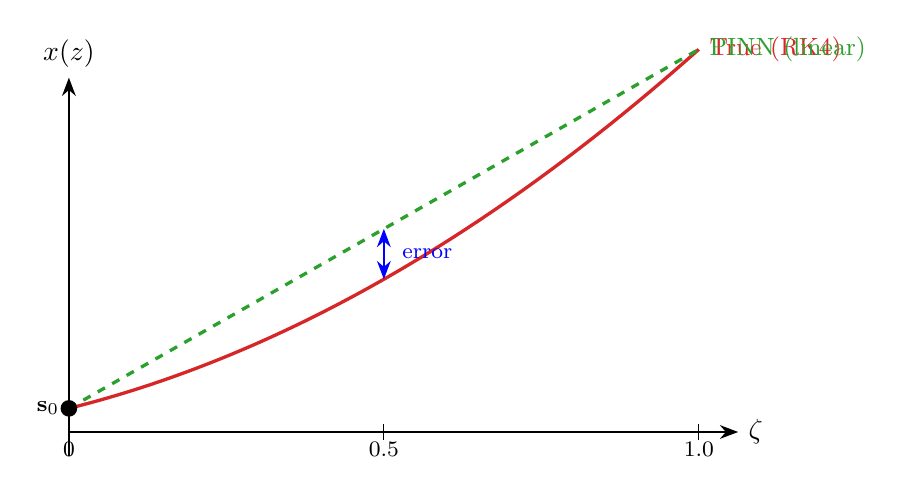
\begin{tikzpicture}[scale=1.0]
  % Axes
  \draw[-Stealth, thick] (0,0) -- (8.5,0) node[right] {$\zfrac$};
  \draw[-Stealth, thick] (0,-0.3) -- (0,4.5) node[above] {$x(z)$};
  % Tick marks
  \foreach \x/\lab in {0/0, 4/0.5, 8/1.0}
    \draw (\x, -0.1) -- (\x, 0.1) node[below=3pt, font=\footnotesize] {\lab};
  % True trajectory (parabolic)
  \draw[very thick, rk4red]
    plot[smooth, domain=0:8, samples=50] (\x, {0.3 + 0.25*\x + 0.04*\x*\x})
    node[right, font=\small] {True (RK4)};
  % Linear PINN
  \draw[very thick, pinngreen, dashed]
    (0, 0.3) -- (8, {0.3 + 0.25*8 + 0.04*8*8})
    node[right, font=\small] {PINN (linear)};
  % Error brace at midpoint
  \pgfmathsetmacro{\truemid}{0.3 + 0.25*4 + 0.04*16}
  \pgfmathsetmacro{\linmid}{0.3 + 0.5*(0.25*8 + 0.04*64)}
  \draw[Stealth-Stealth, thick, blue]
    (4, \truemid) -- (4, \linmid)
    node[midway, right=3pt, font=\footnotesize, text=blue] {error};
  % IC dot
  \fill[black] (0, 0.3) circle (3pt) node[left, font=\footnotesize] {$\vstate_0$};
\end{tikzpicture}
\caption{The PINN's linear output (dashed green) vs.\ the true curved
  trajectory (solid red).  The linear ansatz matches perfectly at $\zfrac=0$
  and $\zfrac=1$ but deviates at intermediate points---this error grows
  quadratically.}
\label{fig:linear_vs_curved}
\end{figure}

\subsubsection{Three Proposed Fixes (V4)}

\paragraph{Fix 1: PINNZFracInput} (recommended).
Add $\zfrac$ and $\dz$ as inputs to the encoder:
\begin{equation}\label{eq:pinnzfrac}
  \vstate(\zfrac) = \vstate_0 + \zfrac \cdot
  \mathcal{N}_\theta\!\bigl(x_0, y_0, \tx{}_0, \ty{}_0, \qop,\, \dz,\,
  \zfrac\bigr)
\end{equation}
Now $\vc$ depends on $\zfrac$, so the output can be nonlinear.  The
IC is still guaranteed: at $\zfrac=0$ the multiplicative factor
zeroes out the correction.

\paragraph{Fix 2: Quadratic Residual.}
Two correction vectors:
\begin{equation}\label{eq:quadratic}
  \vstate(\zfrac) = \vstate_0 + \zfrac\cdot\vc_1 + \zfrac^2\cdot\vc_2
\end{equation}
\noindent The quadratic term captures the dominant bending.  IC is still
exact since both correction terms vanish at $\zfrac=0$.

\paragraph{Fix 3: PDE-Residual (True PINN).}
Use automatic differentiation to compute $d\vstate/d\zfrac$ from the
network, and penalise deviation from the Lorentz ODE directly:
\begin{equation}\label{eq:pde_loss}
  \mathcal{L}_{\mathrm{PDE}} = \frac{1}{N_c}\sum_{j=1}^{N_c}
  \left\|\frac{d\hat{\vstate}}{d\zfrac}\bigg|_{\zfrac_j}
  - \mathbf{f}\bigl(\hat{\vstate}(\zfrac_j),\,\vB(z_j)\bigr)\right\|^2
\end{equation}

% ---------- RK-PINN --------------------------------------------------------
\subsection{RK-PINN (Runge-Kutta PINN) with Collocation}\label{sec:rkpinn}

The RK-PINN combines the residual formulation with a multi-stage structure
inspired by classical Runge-Kutta integrators.

\subsubsection{Classical RK4 Review}

The classical fourth-order Runge-Kutta method evaluates the derivative at
four ``stages'' within each step:
\begin{equation}\label{eq:rk4}
\begin{aligned}
  \mathbf{k}_1 &= h\,\mathbf{f}(z_n,\,\vstate_n) \\
  \mathbf{k}_2 &= h\,\mathbf{f}\!\left(z_n+\tfrac{h}{2},\,
    \vstate_n+\tfrac{\mathbf{k}_1}{2}\right) \\
  \mathbf{k}_3 &= h\,\mathbf{f}\!\left(z_n+\tfrac{h}{2},\,
    \vstate_n+\tfrac{\mathbf{k}_2}{2}\right) \\
  \mathbf{k}_4 &= h\,\mathbf{f}(z_n+h,\,\vstate_n+\mathbf{k}_3) \\[4pt]
  \vstate_{n+1} &= \vstate_n
    + \tfrac{1}{6}\bigl(\mathbf{k}_1 + 2\mathbf{k}_2
    + 2\mathbf{k}_3 + \mathbf{k}_4\bigr)
\end{aligned}
\end{equation}

\subsubsection{RK-PINN Architecture}\label{sec:rkpinn_arch}

The RK-PINN replaces each stage evaluation with a neural-network head.
A shared encoder extracts features from the initial state, and four
separate heads produce corrections at $\zfrac = 0.25,\,0.5,\,0.75,\,1.0$.

\begin{figure}[H]
\centering
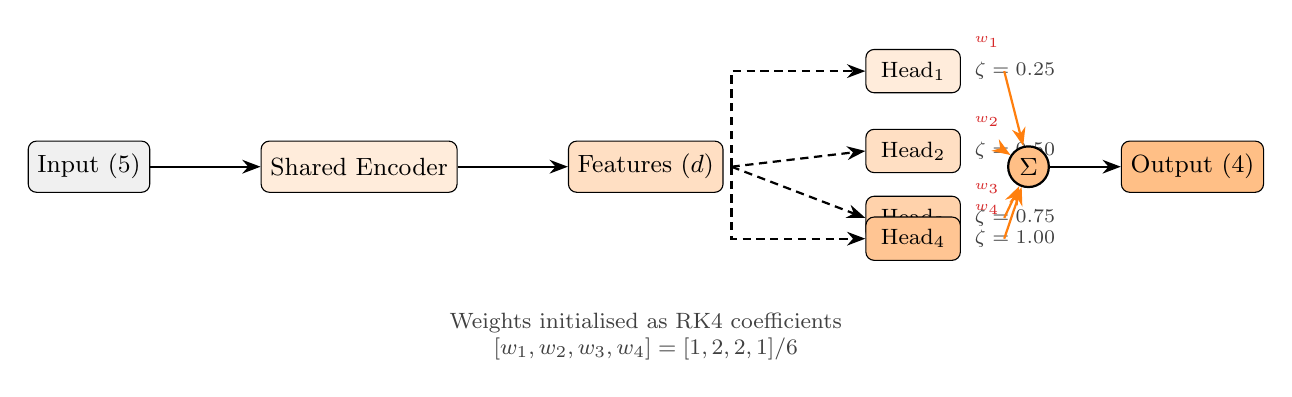
\begin{tikzpicture}[
  node distance=0.7cm and 1.3cm,
  layer/.style={draw, rounded corners=3pt, minimum width=1.4cm,
                minimum height=0.65cm, font=\small},
  head/.style={draw, rounded corners=3pt, minimum width=1.2cm,
               minimum height=0.55cm, font=\footnotesize},
  op/.style={draw, circle, inner sep=2pt, font=\small, thick},
  arrow/.style={-Stealth, thick},
  stage_arrow/.style={-Stealth, thick, densely dashed},
]
  % Input
  \node[layer, fill=lightgray] (in) {Input (5)};
  % Shared encoder
  \node[layer, fill=rkpinnorange!15, right=1.4cm of in,
        minimum width=2.4cm] (enc) {Shared Encoder};
  \draw[arrow] (in) -- (enc);
  % Feature vector
  \node[layer, fill=rkpinnorange!25, right=1.4cm of enc] (feat)
    {Features ($d$)};
  \draw[arrow] (enc) -- (feat);

  % Four stage heads
  \node[head, fill=rkpinnorange!15, above right=0.6cm and 1.8cm of feat]
    (h1) {Head$_1$};
  \node[head, fill=rkpinnorange!25, right=1.8cm of feat, yshift=0.2cm]
    (h2) {Head$_2$};
  \node[head, fill=rkpinnorange!35, right=1.8cm of feat, yshift=-0.65cm]
    (h3) {Head$_3$};
  \node[head, fill=rkpinnorange!45, below right=0.6cm and 1.8cm of feat,
        yshift=0.3cm]
    (h4) {Head$_4$};
  % Labels
  \node[right=0.05cm of h1, font=\scriptsize, text=darkgray]
    {$\zfrac=0.25$};
  \node[right=0.05cm of h2, font=\scriptsize, text=darkgray]
    {$\zfrac=0.50$};
  \node[right=0.05cm of h3, font=\scriptsize, text=darkgray]
    {$\zfrac=0.75$};
  \node[right=0.05cm of h4, font=\scriptsize, text=darkgray]
    {$\zfrac=1.00$};
  % Arrows to heads
  \draw[stage_arrow] (feat.east) ++(0.1,0) |- (h1.west);
  \draw[stage_arrow] (feat.east) ++(0.1,0) -- (h2.west);
  \draw[stage_arrow] (feat.east) ++(0.1,0) -- (h3.west);
  \draw[stage_arrow] (feat.east) ++(0.1,0) |- (h4.west);

  % Weighted sum
  \node[op, fill=rkpinnorange!50, right=3.6cm of feat] (sum) {$\Sigma$};
  % Weight labels
  \node[above right=-0.1cm and 0.05cm of h1, font=\tiny, text=rk4red] {$w_1$};
  \node[above right=-0.1cm and 0.05cm of h2, font=\tiny, text=rk4red] {$w_2$};
  \node[above right=-0.1cm and 0.05cm of h3, font=\tiny, text=rk4red] {$w_3$};
  \node[above right=-0.1cm and 0.05cm of h4, font=\tiny, text=rk4red] {$w_4$};
  % Arrows to sum
  \draw[arrow, rkpinnorange] ($(h1.east)+(0.55,0)$) -- (sum);
  \draw[arrow, rkpinnorange] ($(h2.east)+(0.55,0)$) -- (sum);
  \draw[arrow, rkpinnorange] ($(h3.east)+(0.55,0)$) -- (sum);
  \draw[arrow, rkpinnorange] ($(h4.east)+(0.55,0)$) -- (sum);

  % Output
  \node[layer, fill=rkpinnorange!50, right=0.9cm of sum] (out) {Output (4)};
  \draw[arrow] (sum) -- (out);

  % Label
  \node[below=1.4cm of feat, font=\footnotesize, text=darkgray, align=center]
    {Weights initialised as RK4 coefficients\\
     $[w_1,w_2,w_3,w_4] = [1,2,2,1]/6$};
\end{tikzpicture}
\caption{RK-PINN architecture.  A shared encoder feeds four stage heads,
  each responsible for a different fractional position.  The final output
  is a weighted sum, initialised with RK4 coefficients.}
\label{fig:rkpinn_arch}
\end{figure}

\subsubsection{Mathematical Formulation}

Each head produces a correction at its designated stage position:
\begin{equation}\label{eq:rkpinn_heads}
  \vc_k = \text{Head}_k\!\bigl(\text{features}\bigr),
  \qquad k = 1,2,3,4
\end{equation}

The intermediate states are constructed using the residual formulation:
\begin{equation}\label{eq:rkpinn_states}
  \vstate(\zfrac_k) = \vstate_0 + \zfrac_k \cdot \vc_k,
  \qquad
  \zfrac_k \in \{0.25,\; 0.5,\; 0.75,\; 1.0\}
\end{equation}

The final output is a weighted combination:
\begin{equation}\label{eq:rkpinn_output}
  \hat{\vstate}_{\mathrm{final}} = \vstate_0
  + \sum_{k=1}^{4} w_k\,\vc_k
\end{equation}
where the weights are initialised as $[w_1,w_2,w_3,w_4]=[1,2,2,1]/6$
(the classical RK4 quadrature weights) and are optionally learnable.

% ----------- Collocation theory -------------------------------------------
\subsubsection{Collocation Training}\label{sec:collocation}

Collocation is the technique of enforcing a differential equation at a
discrete set of points.  In the RK-PINN context, we evaluate the model at
$N_c$ fractional positions along the trajectory and compare against
ground-truth data that was pre-computed via RK4 numerical integration.

\paragraph{Collocation points.}
Given a trajectory from $z_0$ to $z_0+\dz$, choose $N_c$ intermediate
evaluation points:
\begin{equation}\label{eq:collocation_points}
  \zfrac_j = \frac{j}{N_c+1}, \qquad j = 1, 2, \ldots, N_c
\end{equation}

At each point, the network prediction $\hat{\vstate}(\zfrac_j)$ is
compared to the RK4 ground truth $\vstate^*(\zfrac_j)$.

\begin{figure}[H]
\centering
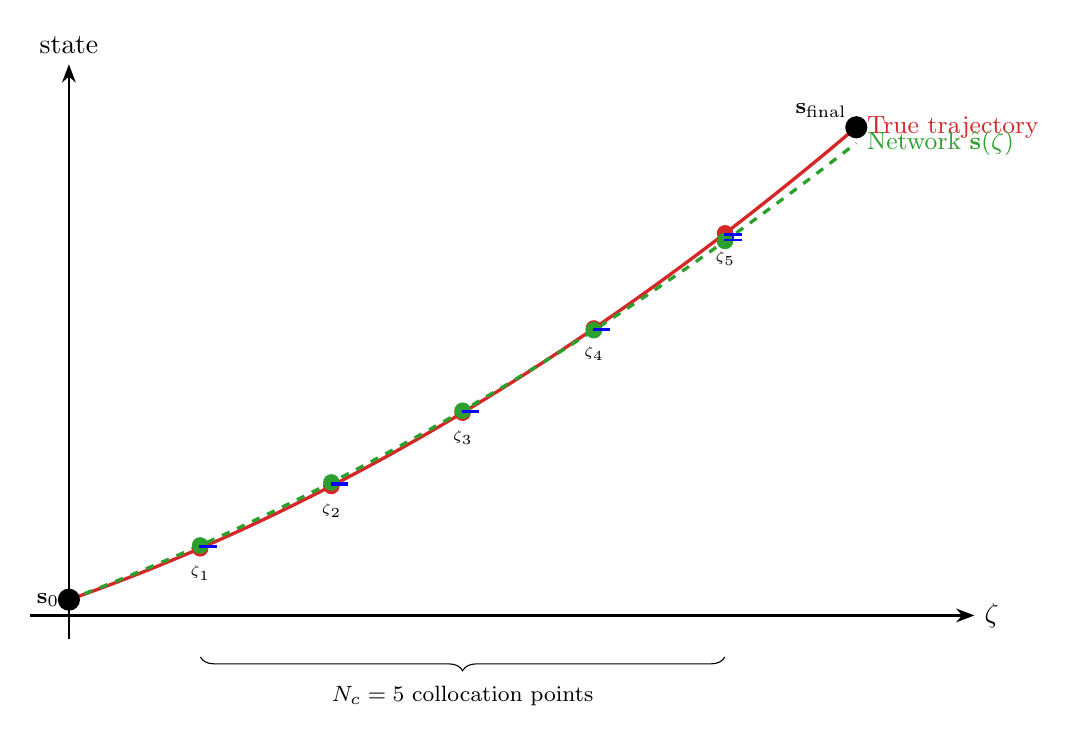
\begin{tikzpicture}[scale=1.0]
  % Trajectory
  \draw[very thick, rk4red]
    plot[smooth, domain=0:10, samples=80]
    (\x, {0.2 + 0.35*\x + 0.025*\x*\x})
    node[right, font=\small] {True trajectory};

  % Network prediction (slightly off)
  \draw[very thick, pinngreen, dashed]
    plot[smooth, domain=0:10, samples=80]
    (\x, {0.2 + 0.38*\x + 0.020*\x*\x})
    node[right, font=\small] {Network $\hat{\vstate}(\zfrac)$};

  % Collocation points
  \foreach \j in {1,...,5}{
    \pgfmathsetmacro{\xp}{\j * 10 / 6}
    \pgfmathsetmacro{\ytrue}{0.2 + 0.35*\xp + 0.025*\xp*\xp}
    \pgfmathsetmacro{\ypred}{0.2 + 0.38*\xp + 0.020*\xp*\xp}
    % True point
    \fill[rk4red] (\xp, \ytrue) circle (3pt);
    % Pred point
    \fill[pinngreen] (\xp, \ypred) circle (3pt);
    % Error bar
    \draw[thick, blue, |-|] (\xp+0.1, \ytrue) -- (\xp+0.1, \ypred);
    % Label
    \node[below=3pt of {(\xp, \ytrue)}, font=\tiny] {$\zfrac_{\j}$};
  }

  % Initial point
  \fill[black] (0, 0.2) circle (4pt)
    node[left, font=\footnotesize] {$\vstate_0$};

  % Endpoint
  \pgfmathsetmacro{\yfinal}{0.2 + 0.35*10 + 0.025*100}
  \fill[black] (10, \yfinal) circle (4pt)
    node[above left, font=\footnotesize] {$\vstate_{\mathrm{final}}$};

  % Axes
  \draw[-Stealth, thick] (-0.5, 0) -- (11.5, 0) node[right] {$\zfrac$};
  \draw[-Stealth, thick] (0, -0.3) -- (0, 7) node[above] {state};

  % Brace
  \draw[decorate, decoration={brace, amplitude=5pt, mirror, raise=15pt}]
    (1.67, 0) -- (8.33, 0)
    node[midway, below=22pt, font=\footnotesize]
    {$N_c = 5$ collocation points};
\end{tikzpicture}
\caption{Supervised collocation.  The network (dashed green) is evaluated
  at $N_c$ intermediate positions and compared against the true RK4
  trajectory (solid red) at each collocation point.  The blue bars show
  the error at each point, which enters the collocation loss.}
\label{fig:collocation}
\end{figure}

\paragraph{Three-part loss function.}
The total PINN / RK-PINN loss combines three terms:

\begin{equation}\label{eq:pinn_loss}
  \boxed{\;
    \mathcal{L}_{\mathrm{PINN}}
    = \lambda_{\IC}\,\mathcal{L}_{\IC}
    + \lambda_{\mathrm{end}}\,\mathcal{L}_{\mathrm{end}}
    + \lambda_{\mathrm{col}}\,\mathcal{L}_{\mathrm{col}}
  \;}
\end{equation}

\begin{enumerate}[nosep]
  \item \textbf{IC loss} (initial condition):
  \begin{equation}\label{eq:ic_loss}
    \mathcal{L}_{\IC} = \frac{1}{B}\sum_{i=1}^{B}
    \bigl\|\hat{\vstate}_i(0) - \vstate_{0,i}\bigr\|^2
  \end{equation}
  With the residual formulation, $\mathcal{L}_{\IC}=0$ exactly.

  \item \textbf{Endpoint loss} (data-driven):
  \begin{equation}\label{eq:end_loss}
    \mathcal{L}_{\mathrm{end}} = \frac{1}{B}\sum_{i=1}^{B}
    \bigl\|\hat{\vstate}_i(1) - \vstate^*_i(1)\bigr\|^2
  \end{equation}

  \item \textbf{Collocation loss} (supervised intermediate points):
  \begin{equation}\label{eq:col_loss}
    \mathcal{L}_{\mathrm{col}} = \frac{1}{B\,N_c}
    \sum_{i=1}^{B}\sum_{j=1}^{N_c}
    \bigl\|\hat{\vstate}_i(\zfrac_j) - \vstate^*_i(\zfrac_j)\bigr\|^2
  \end{equation}
\end{enumerate}

The collocation loss encourages the network to learn the \emph{shape} of
the trajectory, not just the endpoints.  In the RK-PINN, the four stage
heads naturally provide predictions at $\zfrac\in\{0.25, 0.5, 0.75, 1.0\}$,
which serve as four built-in collocation points.

\paragraph{Comparison with PDE collocation.}
In a ``true'' PINN, one would enforce the ODE at collocation points using
automatic differentiation:
\begin{equation}\label{eq:pde_collocation}
  \mathcal{L}_{\mathrm{PDE}} = \frac{1}{N_c}\sum_{j=1}^{N_c}
  \left\|\frac{d\hat{\vstate}}{dz}\bigg|_{z_j}
  - \mathbf{f}\bigl(\hat{\vstate}(z_j),\;\vB(z_j)\bigr)\right\|^2
\end{equation}
This is more principled---it does not require pre-computed trajectory
data---but is harder to train due to the need for second-order gradients
through the magnetic field map.  Our ``supervised collocation''
(Eq.~\ref{eq:col_loss}) is a practical compromise: it uses pre-computed
RK4 data at intermediate points instead of the ODE residual.

\paragraph{Training schedule.}
To stabilise training, a physics-loss warmup was used:
\begin{equation}\label{eq:warmup}
  \lambda_{\mathrm{col}}(t) = \lambda_{\mathrm{col}}^{\max}
  \cdot\min\!\left(1,\;\frac{t}{T_{\mathrm{warmup}}}\right)
\end{equation}
where $t$ is the training step and $T_{\mathrm{warmup}}$ is the warmup
period (typically 2 epochs).  This prevents the physics loss from
dominating early training before the network has learned basic features.

% ----------- Collocation in RK-PINN: why it doesn't help -------------------
\subsubsection{Why Collocation Cannot Fix the Linear Ansatz}
\label{sec:col_cant_fix}

In the V3 experiments, the number of collocation points was varied from
5 to~50.  The results were:
\begin{table}[H]
\centering
\caption{V3 PINN collocation study: increasing points does not help.}
\label{tab:collocation}
\begin{tabular}{@{} r r r @{}}
\toprule
$N_c$ & Pos.\ RMSE (mm) & Slope RMSE \\
\midrule
  5 & 49.4 & 0.000249 \\
 10 & 54.4 & 0.000249 \\
 20 & 52.1 & 0.000251 \\
 50 & 51.8 & 0.000248 \\
\bottomrule
\end{tabular}
\end{table}

The position error is stuck at ${\sim}\SI{50}{\milli\metre}$ regardless of
$N_c$.  This is expected: the linear ansatz
(Eq.~\ref{eq:pinn_residual}) can only produce straight lines in $\zfrac$,
so \emph{adding more supervision points along a line that must be straight
cannot make it curved}.

\begin{figure}[H]
\centering
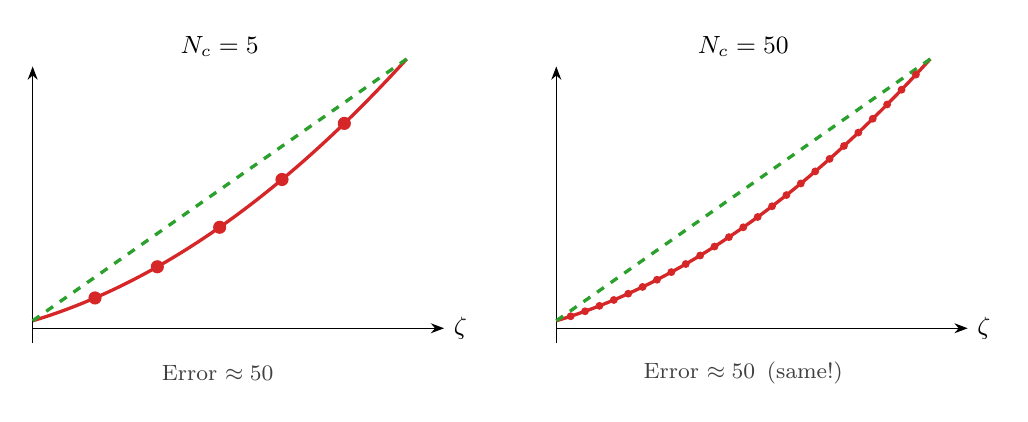
\begin{tikzpicture}[scale=0.95]
  % Two subplots side by side
  % Left: N_c = 5
  \begin{scope}[shift={(0,0)}]
    \draw[-Stealth] (0,0) -- (5.5,0) node[right, font=\small] {$\zfrac$};
    \draw[-Stealth] (0,-0.2) -- (0,3.5);
    \node[above, font=\small\bfseries] at (2.5,3.5) {$N_c=5$};
    % True trajectory
    \draw[very thick, rk4red]
      plot[smooth, domain=0:5, samples=40] (\x, {0.1+0.3*\x+0.08*\x*\x});
    % Linear fit
    \draw[very thick, pinngreen, dashed]
      (0, 0.1) -- (5, {0.1 + 5*(0.3 + 0.08*5)});
    % Collocation dots
    \foreach \j in {1,...,5}{
      \pgfmathsetmacro{\xp}{\j*5/6}
      \pgfmathsetmacro{\yt}{0.1+0.3*\xp+0.08*\xp*\xp}
      \fill[rk4red] (\xp, \yt) circle (2.5pt);
    }
    \node[font=\footnotesize, text=darkgray] at (2.5, -0.6)
      {Error $\approx \SI{50}{\milli\metre}$};
  \end{scope}

  % Right: N_c = 50
  \begin{scope}[shift={(7,0)}]
    \draw[-Stealth] (0,0) -- (5.5,0) node[right, font=\small] {$\zfrac$};
    \draw[-Stealth] (0,-0.2) -- (0,3.5);
    \node[above, font=\small\bfseries] at (2.5,3.5) {$N_c=50$};
    % True trajectory
    \draw[very thick, rk4red]
      plot[smooth, domain=0:5, samples=40] (\x, {0.1+0.3*\x+0.08*\x*\x});
    % Linear fit (same!)
    \draw[very thick, pinngreen, dashed]
      (0, 0.1) -- (5, {0.1 + 5*(0.3 + 0.08*5)});
    % Many collocation dots
    \foreach \j in {1,...,25}{
      \pgfmathsetmacro{\xp}{\j*5/26}
      \pgfmathsetmacro{\yt}{0.1+0.3*\xp+0.08*\xp*\xp}
      \fill[rk4red] (\xp, \yt) circle (1.5pt);
    }
    \node[font=\footnotesize, text=darkgray] at (2.5, -0.6)
      {Error $\approx \SI{50}{\milli\metre}$ (same!)};
  \end{scope}
\end{tikzpicture}
\caption{Increasing collocation points from 5 to 50 does not reduce the
  error.  The linear ansatz (dashed) cannot approximate the curved
  truth (solid), regardless of how many supervision points are provided.}
\label{fig:col_doesnt_help}
\end{figure}

% ============================================================================
\section{Version Timeline}\label{sec:timeline}
% ============================================================================

\begin{table}[H]
\centering
\caption{Summary of the four experiment versions.}
\label{tab:timeline}
\begin{tabular}{@{} l l c l l @{}}
\toprule
Version & Date & $\dz$ & Key change & Outcome \\
\midrule
V1 & Jan 2026 & Fixed \SI{8000}{\milli\metre}
   & First experiments
   & PINNs failed (IC issue) \\
V2 & Jan 2026 & Fixed \SI{8000}{\milli\metre}
   & Residual PINN; shallow-wide MLPs
   & IC fixed; PINNs $2\times$ worse \\
V3 & Jan--Feb 2026 & Variable 500--\SI{12000}{\milli\metre}
   & Variable step-size training
   & MLP ${\sim}\SI{1}{\milli\metre}$; PINN ${\sim}\SI{50}{\milli\metre}$ \\
V4 & Feb 2026 & Variable 500--\SI{12000}{\milli\metre}
   & Width sweep; PINN diagnosis
   & Root cause identified \\
\bottomrule
\end{tabular}
\end{table}

Three critical lessons:
\begin{enumerate}[nosep]
  \item \textbf{V1\,$\to$\,V2:} PINN initial conditions failed because
        the network ignored $\zfrac$.  Fix: residual architecture.
  \item \textbf{V2\,$\to$\,V3:} Fixed-$\dz$ models explode for other step
        sizes ($\sigma_{\dz}\approx10^{-9}$).  Fix: variable $\dz$.
  \item \textbf{V2\,$\to$\,V4:} Residual formula
        $\IC+\zfrac\cdot\vc$ is linear in $\zfrac$---cannot capture
        curved trajectories.  MLPs win because they take $\dz$ as input.
\end{enumerate}

% ============================================================================
\section{V1 Results}\label{sec:v1}
% ============================================================================

53 models trained (14~MLP, 16~PINN, 17~RK-PINN, 6~momentum-binned);
50M training samples; fixed $\dz=\SI{8000}{\milli\metre}$; 10 epochs.

\begin{table}[H]
\centering
\caption{Top V1 models (sorted by validation loss).}
\label{tab:v1}
\begin{tabular}{@{} r l l r r @{}}
\toprule
\# & Model & Type & Params & Val Loss \\
\midrule
1 & mlp\_large\_v1 & MLP & 399K & 0.000445 \\
2 & mlp\_medium & MLP & 101K & 0.000583 \\
3 & rkpinn\_medium\_data\_only & RK-PINN & 101K & 0.000671 \\
4 & mlp\_wide & MLP & 431K & 0.000951 \\
5 & mlp\_medium\_v1 & MLP & 101K & 0.001015 \\
6 & mlp\_wide\_v1 & MLP & 431K & 0.001172 \\
7 & rkpinn\_medium\_pde\_weak & RK-PINN & 101K & 0.001307 \\
8 & mlp\_small & MLP & 18K & 0.001339 \\
9 & mlp\_balanced\_v1 & MLP & 57K & 0.002088 \\
10 & pinn\_small & PINN & 18K & 0.002996 \\
11 & mlp\_tiny & MLP & 5K & 0.003086 \\
12 & pinn\_medium & PINN & 101K & 0.006980 \\
13 & pinn\_medium\_pde\_strong & PINN & 101K & 0.055000 \\
\bottomrule
\end{tabular}
\end{table}

\paragraph{Key issue: PINN IC failure.}
At $\zfrac=0$, the V1 PINN predicted $x=\SI{2768}{\milli\metre}$ when
the input was $x_0=\SI{207}{\milli\metre}$.  The network completely ignored
$\zfrac$; the normalisation statistics had $\sigma_{\dz}\approx10^{-9}$,
so any $\zfrac\neq8000$ produced astronomical values.

% ---- V1 benchmark plots ---------------------------------------------------
\begin{figure}[H]
\centering
\begin{subfigure}[t]{0.48\textwidth}
  \centering
  \includegraphics[width=\textwidth]{V1/benchmarking/plots/fig1_accuracy_comparison.png}
  \caption{Model accuracy comparison.}
\end{subfigure}
\hfill
\begin{subfigure}[t]{0.48\textwidth}
  \centering
  \includegraphics[width=\textwidth]{V1/benchmarking/plots/fig2_error_distribution.png}
  \caption{Error distribution.}
\end{subfigure}

\vspace{8pt}

\begin{subfigure}[t]{0.48\textwidth}
  \centering
  \includegraphics[width=\textwidth]{V1/benchmarking/plots/fig3_accuracy_vs_speed.png}
  \caption{Accuracy vs.\ speed.}
\end{subfigure}
\hfill
\begin{subfigure}[t]{0.48\textwidth}
  \centering
  \includegraphics[width=\textwidth]{V1/benchmarking/plots/fig4_performance_summary.png}
  \caption{Performance summary.}
\end{subfigure}
\caption{V1 benchmarking results.}
\label{fig:v1_bench}
\end{figure}

\begin{figure}[H]
\centering
\begin{subfigure}[t]{0.48\textwidth}
  \centering
  \includegraphics[width=\textwidth]{V1/benchmarking/results/speed_accuracy_tradeoff.png}
  \caption{Speed--accuracy Pareto frontier.}
\end{subfigure}
\hfill
\begin{subfigure}[t]{0.48\textwidth}
  \centering
  \includegraphics[width=\textwidth]{V1/benchmarking/results/timing_distributions.png}
  \caption{Timing distributions.}
\end{subfigure}
\caption{V1 speed--accuracy trade-off.}
\label{fig:v1_speed}
\end{figure}

% ============================================================================
\section{V2 Results}\label{sec:v2}
% ============================================================================

22 models trained (9~MLP, 7~PINN, 6~RK-PINN); residual architecture
introduced; 50M samples; fixed $\dz=\SI{8000}{\milli\metre}$; 20 epochs.

\subsection{MLP Performance}

\begin{table}[H]
\centering
\caption{V2 MLP results (sorted by position error).}
\label{tab:v2_mlp}
\begin{tabular}{@{} l l r r
  r r r @{}}
\toprule
Model & Arch. & Pos (mm) & Pos 90\% (mm) & Slope (mrad)
  & Time ($\mu$s) & Speedup \\
\midrule
shallow\_512\_256 & {[512,256]} & 0.028 & 0.051 & 0.416 & 1.93 & 1.29 \\
shallow\_512     & {[512,512]} & 0.029 & 0.053 & 0.333 & 2.58 & 0.97 \\
shallow\_1024\_256 & {[1024,256]} & 0.031 & 0.060 & 0.678 & 3.56
  & 0.70 \\
shallow\_256     & {[256,256]} & 0.044 & 0.087 & 0.263 & 1.50 & 1.67 \\
single\_1024     & {[1024]}    & 0.062 & 0.149 & 0.026 & 1.86 & 1.34 \\
single\_256      & {[256]}     & 0.065 & 0.135 & 0.017 & 0.83 & 3.00 \\
single\_512      & {[512]}     & 0.068 & 0.139 & 0.013 & 1.03 & 2.44 \\
\bottomrule
\end{tabular}
\end{table}

\subsection{PINN/RK-PINN Performance}

\begin{table}[H]
\centering
\caption{V2 PINN and RK-PINN results: position errors are catastrophic.}
\label{tab:v2_pinn}
\begin{tabular}{@{} l l r r @{}}
\toprule
Model & Type & Pos Error (mm) & Slope (mrad) \\
\midrule
pinn\_v2\_single\_256      & PINN    & 664 & 98.9 \\
pinn\_v2\_shallow\_1024\_256 & PINN  & 830 & 311.0 \\
rkpinn\_v2\_single\_256    & RK-PINN & 816 & 101.0 \\
\bottomrule
\end{tabular}
\end{table}

The residual architecture fixes IC satisfaction but introduces the
linear ansatz limitation (Section~\ref{sec:linear_problem}).

\subsection{Key Finding: Shallow\,$>$\,Deep}

\begin{table}[H]
\centering
\caption{V2 key finding: two wide layers beat five narrow layers.}
\label{tab:shallow_deep}
\begin{tabular}{@{} l r r r @{}}
\toprule
Architecture & Layers & Width & Val Loss \\
\midrule
Deep-narrow (V1) & 5 & 64  & 0.0045 \\
Medium (V1)      & 4 & 128 & 0.0018 \\
\textbf{Shallow-wide (V2)} & \textbf{2} & \textbf{256--512} & \textbf{0.0008} \\
\bottomrule
\end{tabular}
\end{table}

\begin{figure}[H]
\centering
\includegraphics[width=0.7\textwidth]{mlp_width_depth_comparison.png}
\caption{Width vs.\ depth comparison across versions.}
\label{fig:width_depth}
\end{figure}

% ============================================================================
\section{V3 Results}\label{sec:v3}
% ============================================================================

11 models benchmarked in C++ single-sample inference; 100M training samples;
variable $\dz\in[500,\,12000]$~mm.

\subsection{C++ Benchmark}

\begin{table}[H]
\centering
\caption{V3 C++ single-sample benchmark.}
\label{tab:v3}
\begin{tabular}{@{} l l r r r
  r r @{}}
\toprule
Model & Type & Params & Time ($\mu$s) & Speedup
  & Pos RMSE (mm) & Slope RMSE \\
\midrule
RK4 & Numerical & 0 & 85.2 & 1 & 0.0 & 0.0000 \\
Linear & Analytic & 0 & 0.04 & 2131 & 1.6 & 0.0003 \\
Parabolic & Analytic & 0 & 0.09 & 947 & 1.6 & 0.0003 \\
\midrule
MLP deep\_128 & NN & 59K & 65.0 & 1 & 1.0 & 0.0115 \\
MLP shallow\_256 & NN & 101K & 116.2 & 1 & 1.0 & 0.0092 \\
MLP deep\_256 & NN & 233K & 265.7 & 0 & 1.1 & 0.0083 \\
MLP shallow\_512 & NN & 399K & 465.6 & 0 & 1.0 & 0.0094 \\
\midrule
PINN col5 & NN & 69K & 79.3 & 1 & 49.4 & 0.0002 \\
PINN col10 & NN & 69K & 79.3 & 1 & 54.4 & 0.0002 \\
PINN col20 & NN & 69K & 79.4 & 1 & 56.3 & 0.0002 \\
PINN col50 & NN & 69K & 79.4 & 1 & 57.6 & 0.0002 \\
\bottomrule
\end{tabular}
\end{table}

Key observations:
\begin{itemize}[nosep]
  \item MLP position error ${\sim}\SI{1}{\milli\metre}$---much harder
        than V2's \SI{0.03}{\milli\metre} at fixed $\dz$.
  \item PINN position error ${\sim}\SI{50}{\milli\metre}$, but slopes are
        $37\times$ better than MLP (\num{0.00025} vs.\ \num{0.009}).
  \item Increasing $N_c$ from 5 to 50 has no effect (architecture
        bottleneck; see Section~\ref{sec:col_cant_fix}).
  \item C++ single-sample inference (${\sim}\SI{65}{\micro\second}$) is
        comparable to RK4 (\SI{85}{\micro\second}).
\end{itemize}

% ---- V3 analysis plots ---------------------------------------------------
\begin{figure}[H]
\centering
\begin{subfigure}[t]{0.48\textwidth}
  \centering
  \includegraphics[width=\textwidth]{V3/analysis/speed_vs_accuracy.png}
  \caption{Speed vs.\ accuracy.}
\end{subfigure}
\hfill
\begin{subfigure}[t]{0.48\textwidth}
  \centering
  \includegraphics[width=\textwidth]{V3/analysis/timing_comparison.png}
  \caption{Timing comparison.}
\end{subfigure}

\vspace{8pt}

\begin{subfigure}[t]{0.48\textwidth}
  \centering
  \includegraphics[width=\textwidth]{V3/analysis/error_distributions.png}
  \caption{Error distributions.}
\end{subfigure}
\hfill
\begin{subfigure}[t]{0.48\textwidth}
  \centering
  \includegraphics[width=\textwidth]{V3/analysis/component_accuracy.png}
  \caption{Component-level accuracy.}
\end{subfigure}
\caption{V3 analysis plots.}
\label{fig:v3_analysis}
\end{figure}

\begin{figure}[H]
\centering
\includegraphics[width=0.65\textwidth]{V3/analysis/error_vs_kinematics.png}
\caption{V3 error dependence on momentum and $\dz$.}
\label{fig:v3_kinematics}
\end{figure}

\subsection{Component-Level Accuracy (MLP shallow\_512)}

\begin{table}[H]
\centering
\caption{Per-component RMSE for the best V3 MLP.}
\label{tab:v3_components}
\begin{tabular}{@{} l r @{}}
\toprule
Component & RMSE \\
\midrule
$x$ position & 0.80\;\text{mm} \\
$y$ position & 0.53\;\text{mm} \\
$\tx$ slope  & 0.0076 \\
$\ty$ slope  & 0.0056 \\
\bottomrule
\end{tabular}
\end{table}

% ============================================================================
\section{V4 Results}\label{sec:v4}
% ============================================================================

V4 pursues two parallel tracks: MLP width scaling and PINN architecture
diagnosis.

\subsection{MLP Width Sweep}

\begin{table}[H]
\centering
\caption{V4 planned width sweep configurations.}
\label{tab:v4_sweep}
\begin{tabular}{@{} l l r r l @{}}
\toprule
Model & Architecture & Est.\ Params & Est.\ Time ($\mu$s) & Status \\
\midrule
mlp\_v4\_1L\_512  & {[512]}  & 5K   & ${\sim}4$  & Training \\
mlp\_v4\_1L\_1024 & {[1024]} & 10K  & ${\sim}8$  & Training \\
mlp\_v4\_1L\_2048 & {[2048]} & 20K  & ${\sim}16$ & Training \\
mlp\_v4\_1L\_4096 & {[4096]} & 41K  & ${\sim}32$ & Training \\
mlp\_v4\_2L\_1024 & {[1024,512]} & 524K & --- & Planned \\
mlp\_v4\_2L\_2048 & {[2048,1024]} & 2.1M & --- & Planned \\
\bottomrule
\end{tabular}
\end{table}

\subsection{PINN Diagnosis}

Root cause of PINN failure confirmed: the encoder lacks $\zfrac$ as input,
forcing a linear output (Section~\ref{sec:linear_problem}).

\begin{figure}[H]
\centering
\begin{subfigure}[t]{0.48\textwidth}
  \centering
  \includegraphics[width=\textwidth]{V4/p1_zfrac_linearity.png}
  \caption{PINN output is perfectly linear in $\zfrac$.}
\end{subfigure}
\hfill
\begin{subfigure}[t]{0.48\textwidth}
  \centering
  \includegraphics[width=\textwidth]{V4/pinn_trajectory_comparison.png}
  \caption{PINN (linear) vs.\ RK4 (curved).}
\end{subfigure}
\caption{V4 diagnosis: the PINN's linear ansatz cannot capture trajectory
  curvature.}
\label{fig:v4_diagnosis}
\end{figure}

\begin{figure}[H]
\centering
\includegraphics[width=0.6\textwidth]{V4/pinn_training_curves.png}
\caption{V4 training curves: PINN vs.\ MLP.}
\label{fig:v4_training}
\end{figure}

Three proposed fixes with expected performance:

\begin{table}[H]
\centering
\caption{V4 proposed PINN fixes.}
\label{tab:v4_fixes}
\begin{tabular}{@{} l l r @{}}
\toprule
Fix & Idea & Expected Pos.\ Error \\
\midrule
PINNZFracInput & Add $\zfrac$ as 7th encoder input
  & $<\SI{1}{\milli\metre}$ \\
QuadraticResidual & $\IC + \zfrac\cdot\vc_1 + \zfrac^2\cdot\vc_2$
  & $<\SI{5}{\milli\metre}$ \\
PDE-Residual & Autodiff Lorentz loss
  & $<\SI{0.3}{\milli\metre}$ \\
\bottomrule
\end{tabular}
\end{table}

% ============================================================================
\section{Cross-Version Comparison}\label{sec:cross}
% ============================================================================

\subsection{Position Accuracy Evolution}

\begin{table}[H]
\centering
\caption{Best position errors across versions.}
\label{tab:cross_pos}
\begin{tabular}{@{} l r l c r @{}}
\toprule
Version & Best MLP (mm) & Best PINN & $\dz$ & Models \\
\midrule
V1 & {${\sim}0.5$}   & broken (IC) & Fixed & 53 \\
V2 & 0.028            & \SI{664}{\milli\metre} & Fixed & 22 \\
V3 & 0.960            & \SI{49}{\milli\metre}  & Variable & 8 \\
V4 & {in progress}    & in progress & Variable & 24+ \\
\bottomrule
\end{tabular}
\end{table}

\begin{figure}[H]
\centering
\includegraphics[width=0.65\textwidth]{cross_version_position_error.png}
\caption{Position error evolution across versions.}
\label{fig:cross_version}
\end{figure}

\subsection{Speed Evolution}

\begin{table}[H]
\centering
\caption{Best inference speed across versions.}
\label{tab:cross_speed}
\begin{tabular}{@{} l r r l @{}}
\toprule
Version & Best Time ($\mu$s) & vs.\ RK4 & Timing mode \\
\midrule
V1 & 1.10 & 2.3 & Python batched \\
V2 & 0.83 & 3.0 & Python batched \\
V3 & 65.0 & 1.3 & C++ single-sample \\
V4 & {${\sim}8$} & {${\sim}10$} & C++ single (est.) \\
\bottomrule
\end{tabular}
\end{table}

Note: V1/V2 timings are Python with batch size ${\sim}10\text{K}$
(misleadingly fast); V3/V4 use C++ single-sample timing.

% ============================================================================
\section{C++ Benchmark: Traditional Extrapolators}\label{sec:cpp}
% ============================================================================

\begin{table}[H]
\centering
\caption{Traditional C++ extrapolators in LHCb.}
\label{tab:cpp}
\begin{tabular}{@{} l l r r l @{}}
\toprule
Extrapolator & Type & Time ($\mu$s) & Pos Error (mm) & Note \\
\midrule
CashKarp (RK4) & Numerical & 2.50 & 0.0  & Ground truth \\
BogackiShampine3 & RK3     & 2.40 & 0.10 & Best speed/accuracy \\
Verner9        & RK9       & 2.52 & 0.08 & Highest precision \\
Tsitouras5     & RK5       & 2.75 & {---}  & Balanced \\
Herab          & Helix     & 1.95 & 5.1  & Fast seeding \\
Kisel          & Analytical & 1.50 & 39.8 & Do not use \\
\bottomrule
\end{tabular}
\end{table}

% ============================================================================
\section{Physics Exploration Plots}\label{sec:physics_plots}
% ============================================================================

Additional physics-related insights from the exploration notebooks.

\begin{figure}[H]
\centering
\begin{subfigure}[t]{0.48\textwidth}
  \centering
  \includegraphics[width=\textwidth]{physics_trajectories.png}
  \caption{Example charged particle trajectories.}
\end{subfigure}
\hfill
\begin{subfigure}[t]{0.48\textwidth}
  \centering
  \includegraphics[width=\textwidth]{physics_curvature.png}
  \caption{Curvature vs.\ position in the field.}
\end{subfigure}

\vspace{8pt}

\begin{subfigure}[t]{0.48\textwidth}
  \centering
  \includegraphics[width=\textwidth]{physics_momentum_scaling.png}
  \caption{Bending vs.\ momentum ($\propto 1/p$).}
\end{subfigure}
\hfill
\begin{subfigure}[t]{0.48\textwidth}
  \centering
  \includegraphics[width=\textwidth]{physics_collocation_view.png}
  \caption{Collocation points along a trajectory.}
\end{subfigure}
\caption{Physics exploration: trajectories, curvature, momentum scaling,
  and collocation visualisation.}
\label{fig:physics_explore}
\end{figure}

\begin{figure}[H]
\centering
\begin{subfigure}[t]{0.48\textwidth}
  \centering
  \includegraphics[width=\textwidth]{physics_energy_conservation.png}
  \caption{Energy conservation check.}
\end{subfigure}
\hfill
\begin{subfigure}[t]{0.48\textwidth}
  \centering
  \includegraphics[width=\textwidth]{physics_poly_order.png}
  \caption{Polynomial order needed for trajectory fit.}
\end{subfigure}
\caption{Further physics validation.}
\label{fig:physics_extra}
\end{figure}

\begin{figure}[H]
\centering
\begin{subfigure}[t]{0.48\textwidth}
  \centering
  \includegraphics[width=\textwidth]{physics_Fdotv.png}
  \caption{$\vec{F}\cdot\vec{v}$ check (should be zero).}
\end{subfigure}
\hfill
\begin{subfigure}[t]{0.48\textwidth}
  \centering
  \includegraphics[width=\textwidth]{pinn_vs_mlp_v3.png}
  \caption{PINN vs.\ MLP comparison (V3).}
\end{subfigure}
\caption{Force orthogonality and model comparison.}
\label{fig:physics_force}
\end{figure}

% ============================================================================
\section{Conclusions and Next Steps}\label{sec:conclusion}
% ============================================================================

\subsection{What Works}

\begin{enumerate}[nosep]
  \item \textbf{MLPs are effective track extrapolators.}  With 2~hidden
    layers of 512~neurons, position errors are sub-mm (fixed~$\dz$) and
    ${\sim}\SI{1}{\milli\metre}$ (variable~$\dz$).
  \item \textbf{Shallow-wide beats deep-narrow.}  Two layers with
    256--1024 neurons outperform five layers with 64--128.
  \item \textbf{Variable~$\dz$ is essential} for deployment.  Fixed-$\dz$
    models diverge for any other step size.
  \item \textbf{PINNs achieve excellent slopes} (\num{0.0003} vs.\
    \num{0.009}), but position accuracy depends on sufficient architectural
    capacity.
\end{enumerate}

\subsection{What Doesn't Work Yet}

\begin{enumerate}[nosep]
  \item PINN residual with linear $\zfrac$-scaling (cannot capture curvature).
  \item Deep-narrow networks (less accurate and often slower).
  \item Single-sample C++ inference (comparable to RK4 at
    ${\sim}\SI{65}{\micro\second}$).
\end{enumerate}

\subsection{Next Steps}

\begin{table}[H]
\centering
\caption{Prioritised next steps.}
\label{tab:next}
\begin{tabular}{@{} l l l @{}}
\toprule
Priority & Task & Expected impact \\
\midrule
High & V4 width sweep (1L up to 4096) & Optimal width for $<\SI{85}{\micro\second}$ \\
High & PINNZFracInput training & MLP positions + PINN slopes \\
Medium & Float32 inference & ${\sim}2\times$ speed \\
Medium & SIMD/batched C++ & $2$--$50\times$ speed \\
Low & True PDE-residual PINN & No trajectory data needed \\
Low & Momentum-binned models & Better per-bin accuracy \\
\bottomrule
\end{tabular}
\end{table}

\subsection{The Big Picture}

\begin{table}[H]
\centering
\caption{Where neural networks sit in the extrapolation landscape.}
\label{tab:big_picture}
\begin{tabular}{@{} l c c l @{}}
\toprule
Extrapolator & Pos.\ Error & Speed & Physics \\
\midrule
Parabolic & \SI{1.6}{\milli\metre} & $947\times$ RK4 & Minimal \\
MLP (V3 best) & ${\sim}\SI{1}{\milli\metre}$ & $1.3\times$ RK4 & Learned from data \\
RK4 & 0 (truth) & Baseline & Full \\
PINNZFracInput (V4) & $<\SI{1}{\milli\metre}$ & ${\sim}1.2\times$ RK4
  & Partially enforced \\
\bottomrule
\end{tabular}
\end{table}

With wider architectures (V4) and proper PINN design, sub-millimetre
accuracy at $2$--$10\times$ the speed of RK4 appears achievable.

\vfill
\noindent\rule{\textwidth}{0.4pt}\\[4pt]
{\small\itshape Document generated: February 23, 2026.\\
Source: V1--V4 documentation, CSV results, benchmark data, and analysis
notebooks in \texttt{experiments/next\_generation/}.}

\end{document}
